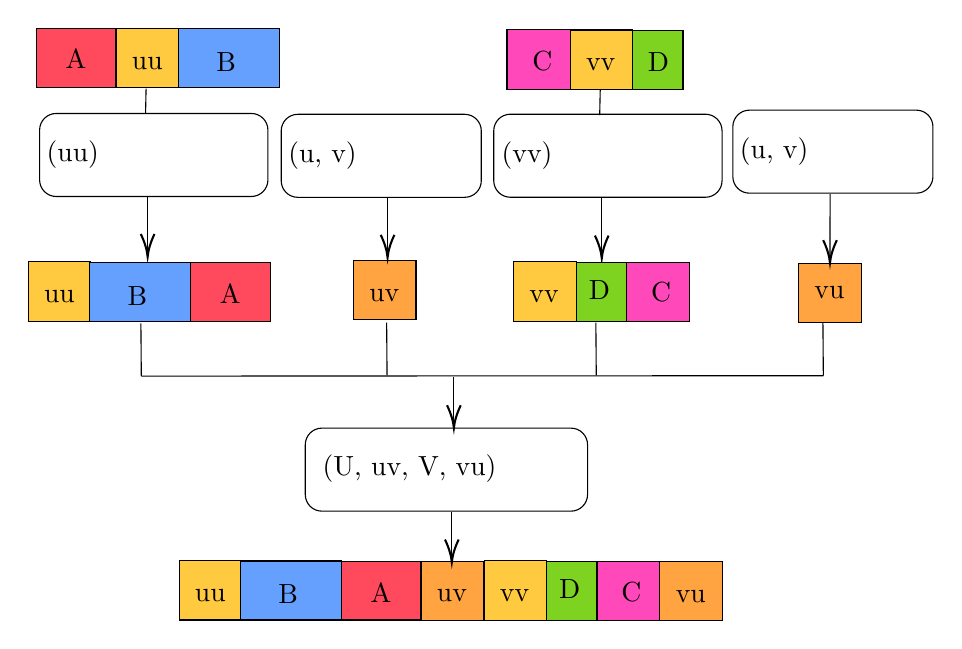
\begin{tikzpicture}[x=0.75pt,y=0.75pt,yscale=-1,xscale=1]
%uncomment if require: \path (0,300); %set diagram left start at 0, and has height of 300

%Shape: Rectangle [id:dp23098094173558026] 
\draw  [fill={rgb, 255:red, 255; green, 73; blue, 92 }  ,fill opacity=1 ] (180.6,2.79) -- (219.02,2.79) -- (219.02,31.54) -- (180.6,31.54) -- cycle ;
%Shape: Rectangle [id:dp6390512458709207] 
\draw  [fill={rgb, 255:red, 102; green, 160; blue, 255 }  ,fill opacity=1 ] (249.19,3.12) -- (297.8,3.12) -- (297.8,31.54) -- (249.19,31.54) -- cycle ;
%Shape: Rectangle [id:dp6196376467227851] 
\draw  [fill={rgb, 255:red, 255; green, 202; blue, 64 }  ,fill opacity=1 ] (219.02,2.87) -- (249.19,2.87) -- (249.19,31.54) -- (219.02,31.54) -- cycle ;
%Shape: Rectangle [id:dp3986048597954386] 
\draw  [fill={rgb, 255:red, 255; green, 202; blue, 64 }  ,fill opacity=1 ] (176.72,115.25) -- (206.89,115.25) -- (206.89,143.91) -- (176.72,143.91) -- cycle ;
%Rounded Rect [id:dp24586206145017386] 
\draw   (182.2,51.86) .. controls (182.2,47.44) and (185.78,43.86) .. (190.2,43.86) -- (284.2,43.86) .. controls (288.62,43.86) and (292.2,47.44) .. (292.2,51.86) -- (292.2,75.86) .. controls (292.2,80.28) and (288.62,83.86) .. (284.2,83.86) -- (190.2,83.86) .. controls (185.78,83.86) and (182.2,80.28) .. (182.2,75.86) -- cycle ;
%Straight Lines [id:da9018859190325679] 
\draw    (233.5,31.88) -- (233.25,43.88) ;
%Straight Lines [id:da2681283034938149] 
\draw    (234.25,83.88) -- (234.25,110.88) ;
\draw [shift={(234.25,112.88)}, rotate = 270] [color={rgb, 255:red, 0; green, 0; blue, 0 }  ][line width=0.75]    (10.93,-3.29) .. controls (6.95,-1.4) and (3.31,-0.3) .. (0,0) .. controls (3.31,0.3) and (6.95,1.4) .. (10.93,3.29)   ;
%Shape: Rectangle [id:dp2680038252592908] 
\draw  [fill={rgb, 255:red, 255; green, 73; blue, 187 }  ,fill opacity=1 ] (407.4,3.54) -- (437.82,3.54) -- (437.82,32.29) -- (407.4,32.29) -- cycle ;
%Shape: Rectangle [id:dp12567524429701304] 
\draw  [fill={rgb, 255:red, 126; green, 211; blue, 33 }  ,fill opacity=1 ] (467.99,3.88) -- (492.2,3.88) -- (492.2,32.29) -- (467.99,32.29) -- cycle ;
%Shape: Rectangle [id:dp8386124850301758] 
\draw  [fill={rgb, 255:red, 255; green, 202; blue, 64 }  ,fill opacity=1 ] (437.82,3.63) -- (467.99,3.63) -- (467.99,32.29) -- (437.82,32.29) -- cycle ;
%Shape: Rectangle [id:dp7066902866408097] 
\draw  [fill={rgb, 255:red, 255; green, 202; blue, 64 }  ,fill opacity=1 ] (410.62,115.23) -- (440.79,115.23) -- (440.79,143.89) -- (410.62,143.89) -- cycle ;
%Rounded Rect [id:dp49539254762727447] 
\draw   (401,52.22) .. controls (401,47.8) and (404.58,44.22) .. (409,44.22) -- (503,44.22) .. controls (507.42,44.22) and (511,47.8) .. (511,52.22) -- (511,76.22) .. controls (511,80.63) and (507.42,84.22) .. (503,84.22) -- (409,84.22) .. controls (404.58,84.22) and (401,80.63) .. (401,76.22) -- cycle ;
%Straight Lines [id:da3433345503689891] 
\draw    (452.3,32.63) -- (452.05,44.63) ;
%Straight Lines [id:da7086447624872888] 
\draw    (453.05,84.63) -- (453.05,111.63) ;
\draw [shift={(453.05,113.63)}, rotate = 270] [color={rgb, 255:red, 0; green, 0; blue, 0 }  ][line width=0.75]    (10.93,-3.29) .. controls (6.95,-1.4) and (3.31,-0.3) .. (0,0) .. controls (3.31,0.3) and (6.95,1.4) .. (10.93,3.29)   ;
%Shape: Rectangle [id:dp7108227182425932] 
\draw  [fill={rgb, 255:red, 102; green, 160; blue, 255 }  ,fill opacity=1 ] (206.39,115.48) -- (255,115.48) -- (255,143.89) -- (206.39,143.89) -- cycle ;
%Shape: Rectangle [id:dp6562117726236578] 
\draw  [fill={rgb, 255:red, 255; green, 73; blue, 92 }  ,fill opacity=1 ] (254.85,115.55) -- (293.28,115.55) -- (293.28,143.88) -- (254.85,143.88) -- cycle ;
%Shape: Rectangle [id:dp00475439694432378] 
\draw  [fill={rgb, 255:red, 126; green, 211; blue, 33 }  ,fill opacity=1 ] (440.79,115.48) -- (465,115.48) -- (465,143.89) -- (440.79,143.89) -- cycle ;
%Shape: Rectangle [id:dp7724716404431173] 
\draw  [fill={rgb, 255:red, 255; green, 73; blue, 187 }  ,fill opacity=1 ] (465,115.48) -- (495.42,115.48) -- (495.42,143.91) -- (465,143.91) -- cycle ;
%Rounded Rect [id:dp6351032187155639] 
\draw   (298.6,52.26) .. controls (298.6,47.84) and (302.18,44.26) .. (306.6,44.26) -- (387,44.26) .. controls (391.42,44.26) and (395,47.84) .. (395,52.26) -- (395,76.26) .. controls (395,80.68) and (391.42,84.26) .. (387,84.26) -- (306.6,84.26) .. controls (302.18,84.26) and (298.6,80.68) .. (298.6,76.26) -- cycle ;
%Rounded Rect [id:dp886163672942809] 
\draw   (516.2,50.26) .. controls (516.2,45.84) and (519.78,42.26) .. (524.2,42.26) -- (604.6,42.26) .. controls (609.02,42.26) and (612.6,45.84) .. (612.6,50.26) -- (612.6,74.26) .. controls (612.6,78.68) and (609.02,82.26) .. (604.6,82.26) -- (524.2,82.26) .. controls (519.78,82.26) and (516.2,78.68) .. (516.2,74.26) -- cycle ;
%Shape: Rectangle [id:dp5872936158482377] 
\draw  [fill={rgb, 255:red, 255; green, 164; blue, 64 }  ,fill opacity=1 ] (333.37,114.61) -- (363.54,114.61) -- (363.54,143.27) -- (333.37,143.27) -- cycle ;
%Shape: Rectangle [id:dp1060558952290429] 
\draw  [fill={rgb, 255:red, 255; green, 164; blue, 64 }  ,fill opacity=1 ] (547.84,116.07) -- (578.01,116.07) -- (578.01,144.74) -- (547.84,144.74) -- cycle ;
%Straight Lines [id:da8424676187890304] 
\draw    (349.85,84.28) -- (349.85,111.28) ;
\draw [shift={(349.85,113.28)}, rotate = 270] [color={rgb, 255:red, 0; green, 0; blue, 0 }  ][line width=0.75]    (10.93,-3.29) .. controls (6.95,-1.4) and (3.31,-0.3) .. (0,0) .. controls (3.31,0.3) and (6.95,1.4) .. (10.93,3.29)   ;
%Straight Lines [id:da923579018004108] 
\draw    (563.05,82.68) -- (563,113.83) ;
\draw [shift={(563,115.83)}, rotate = 270.09] [color={rgb, 255:red, 0; green, 0; blue, 0 }  ][line width=0.75]    (10.93,-3.29) .. controls (6.95,-1.4) and (3.31,-0.3) .. (0,0) .. controls (3.31,0.3) and (6.95,1.4) .. (10.93,3.29)   ;
%Rounded Rect [id:dp897495190590268] 
\draw   (310.2,203.46) .. controls (310.2,199.04) and (313.78,195.46) .. (318.2,195.46) -- (438.2,195.46) .. controls (442.62,195.46) and (446.2,199.04) .. (446.2,203.46) -- (446.2,227.46) .. controls (446.2,231.88) and (442.62,235.46) .. (438.2,235.46) -- (318.2,235.46) .. controls (313.78,235.46) and (310.2,231.88) .. (310.2,227.46) -- cycle ;
%Straight Lines [id:da7028708333591134] 
\draw    (381.8,171) -- (381.8,193.4) ;
\draw [shift={(381.8,195.4)}, rotate = 270] [color={rgb, 255:red, 0; green, 0; blue, 0 }  ][line width=0.75]    (10.93,-3.29) .. controls (6.95,-1.4) and (3.31,-0.3) .. (0,0) .. controls (3.31,0.3) and (6.95,1.4) .. (10.93,3.29)   ;
%Straight Lines [id:da9585719803696012] 
\draw    (231.2,170.4) -- (559.8,170.2) ;
%Straight Lines [id:da6415545775583412] 
\draw    (231,145) -- (231.2,170.4) ;
%Straight Lines [id:da43658433388512063] 
\draw    (349.4,144.6) -- (349.6,170) ;
%Straight Lines [id:da11332243007590326] 
\draw    (450.2,144.6) -- (450.4,170) ;
%Straight Lines [id:da6374722510529054] 
\draw    (559.6,144.8) -- (559.8,170.2) ;
%Shape: Rectangle [id:dp4857436011752162] 
\draw  [fill={rgb, 255:red, 255; green, 202; blue, 64 }  ,fill opacity=1 ] (249.39,259.25) -- (279.55,259.25) -- (279.55,287.91) -- (249.39,287.91) -- cycle ;
%Shape: Rectangle [id:dp9481406925397475] 
\draw  [fill={rgb, 255:red, 255; green, 202; blue, 64 }  ,fill opacity=1 ] (396.38,259.41) -- (426.55,259.41) -- (426.55,288.08) -- (396.38,288.08) -- cycle ;
%Shape: Rectangle [id:dp05525262459567826] 
\draw  [fill={rgb, 255:red, 102; green, 160; blue, 255 }  ,fill opacity=1 ] (279.06,259.48) -- (327.67,259.48) -- (327.67,287.89) -- (279.06,287.89) -- cycle ;
%Shape: Rectangle [id:dp6481351134371125] 
\draw  [fill={rgb, 255:red, 255; green, 73; blue, 92 }  ,fill opacity=1 ] (327.52,259.55) -- (365.95,259.55) -- (365.95,287.88) -- (327.52,287.88) -- cycle ;
%Shape: Rectangle [id:dp20389547363110272] 
\draw  [fill={rgb, 255:red, 126; green, 211; blue, 33 }  ,fill opacity=1 ] (426.55,259.66) -- (450.76,259.66) -- (450.76,288.08) -- (426.55,288.08) -- cycle ;
%Shape: Rectangle [id:dp09319548306175252] 
\draw  [fill={rgb, 255:red, 255; green, 73; blue, 187 }  ,fill opacity=1 ] (450.76,259.66) -- (481.18,259.66) -- (481.18,288.09) -- (450.76,288.09) -- cycle ;
%Shape: Rectangle [id:dp6861148329165587] 
\draw  [fill={rgb, 255:red, 255; green, 164; blue, 64 }  ,fill opacity=1 ] (365.95,259.55) -- (396.11,259.55) -- (396.11,288) -- (365.95,288) -- cycle ;
%Shape: Rectangle [id:dp46764729582654896] 
\draw  [fill={rgb, 255:red, 255; green, 164; blue, 64 }  ,fill opacity=1 ] (481.05,259.53) -- (511.22,259.53) -- (511.22,288.19) -- (481.05,288.19) -- cycle ;
%Straight Lines [id:da07592915614737505] 
\draw    (380.8,235.67) -- (380.8,258.07) ;
\draw [shift={(380.8,260.07)}, rotate = 270] [color={rgb, 255:red, 0; green, 0; blue, 0 }  ][line width=0.75]    (10.93,-3.29) .. controls (6.95,-1.4) and (3.31,-0.3) .. (0,0) .. controls (3.31,0.3) and (6.95,1.4) .. (10.93,3.29)   ;

% Text Node
\draw (193.52,11.84) node [anchor=north west][inner sep=0.75pt]   [align=left] {A};
% Text Node
\draw (266.15,13.44) node [anchor=north west][inner sep=0.75pt]   [align=left] {B};
% Text Node
\draw (225.41,15.62) node [anchor=north west][inner sep=0.75pt]   [align=left] {uu};
% Text Node
\draw (183.11,128) node [anchor=north west][inner sep=0.75pt]   [align=left] {uu};
% Text Node
\draw (184.34,55.66) node [anchor=north west][inner sep=0.75pt]   [align=left] {\ETmovetofront(uu)};
% Text Node
\draw (418.32,12.6) node [anchor=north west][inner sep=0.75pt]   [align=left] {C};
% Text Node
\draw (473.95,13.2) node [anchor=north west][inner sep=0.75pt]   [align=left] {D};
% Text Node
\draw (444.21,16.38) node [anchor=north west][inner sep=0.75pt]   [align=left] {vv};
% Text Node
\draw (416.96,127.76) node [anchor=north west][inner sep=0.75pt]   [align=left] {vv};
% Text Node
\draw (403.54,56.42) node [anchor=north west][inner sep=0.75pt]   [align=left] {\ETmovetofront(vv)};
% Text Node
\draw (223.35,125.8) node [anchor=north west][inner sep=0.75pt]   [align=left] {B};
% Text Node
\draw (267.78,125.18) node [anchor=north west][inner sep=0.75pt]   [align=left] {A};
% Text Node
\draw (445.55,123.2) node [anchor=north west][inner sep=0.75pt]   [align=left] {D};
% Text Node
\draw (475.52,124.2) node [anchor=north west][inner sep=0.75pt]   [align=left] {C};
% Text Node
\draw (300.74,56.06) node [anchor=north west][inner sep=0.75pt]   [align=left] {\treapCreate(u, v)};
% Text Node
\draw (518.34,54.06) node [anchor=north west][inner sep=0.75pt]   [align=left] {\treapCreate(u, v)};
% Text Node
\draw (339.76,127.36) node [anchor=north west][inner sep=0.75pt]   [align=left] {uv};
% Text Node
\draw (554.23,125.82) node [anchor=north west][inner sep=0.75pt]   [align=left] {vu};
% Text Node
\draw (317.34,207.26) node [anchor=north west][inner sep=0.75pt]   [align=left] {\treapJoin(U, uv, V, vu)};
% Text Node
\draw (255.78,272) node [anchor=north west][inner sep=0.75pt]   [align=left] {uu};
% Text Node
\draw (402.72,271.94) node [anchor=north west][inner sep=0.75pt]   [align=left] {vv};
% Text Node
\draw (296.01,269.8) node [anchor=north west][inner sep=0.75pt]   [align=left] {B};
% Text Node
\draw (340.45,269.18) node [anchor=north west][inner sep=0.75pt]   [align=left] {A};
% Text Node
\draw (431.3,267.38) node [anchor=north west][inner sep=0.75pt]   [align=left] {D};
% Text Node
\draw (461.28,268.38) node [anchor=north west][inner sep=0.75pt]   [align=left] {C};
% Text Node
\draw (372.34,271.99) node [anchor=north west][inner sep=0.75pt]   [align=left] {uv};
% Text Node
\draw (487.44,272.28) node [anchor=north west][inner sep=0.75pt]   [align=left] {vu};


\end{tikzpicture}

